\section{Regressão Robusta}

\subsection{Leituras Recomendadas}
\begin{frame}{Regressão Robusta - Leituras Recomendadas}
    \begin{vfilleditems}
        \item \textcite{gelman2013bayesian} - Capítulo 17: Models for robust inference
        \item \textcite{mcelreath2020statistical} - Capítulo 12: Monsters and Mixtures
        \item \textcite{gelman2020regression}:
        \begin{vfilleditems}
            \item Capítulo 15, Seção 15.6: Robust regression using the t model
            \item Capítulo 15, Seção 15.8: Going beyond generalized linear models
        \end{vfilleditems}
        \item \textcite{storopoli2021estatisticabayesianaR} - Regressão Robusta
        \item Tutorial de \texttt{brms} de \textcite{burknerAdvancedBayesianMultilevel2018}
    \end{vfilleditems}
\end{frame}

\begin{frame}{Modelos Robustos\footnote{\href{https://github.com/allisonhorst/stats-illustrations}{digura de Allison Horst (CC-BY-4.0)}}}
    \begin{columns}
        \begin{column}{0.6\textwidth}
            Quase sempre nossos dados no mundo real são bem estranhos.
            \vfill
            Por conveniência usamos modelos simples. Mas sempre se
            pergunte. De que maneiras a inferência da posterior depende de:
            \vfill
            \begin{vfilleditems}
                \item Observações extremas (\textit{outliers})?
                \item Suposições de modelo não-acessíveis?
            \end{vfilleditems}
            \vfill
            Além disso vamos usar \textbf{exclusivamente} o
            \href{https://paul-buerkner.github.io/brms/}{\texttt{brms}}
            ao invés do \href{http://mc-stan.org/rstanarm/}{\texttt{rstanarm}}.
        \end{column}
        \begin{column}{0.4\textwidth}
            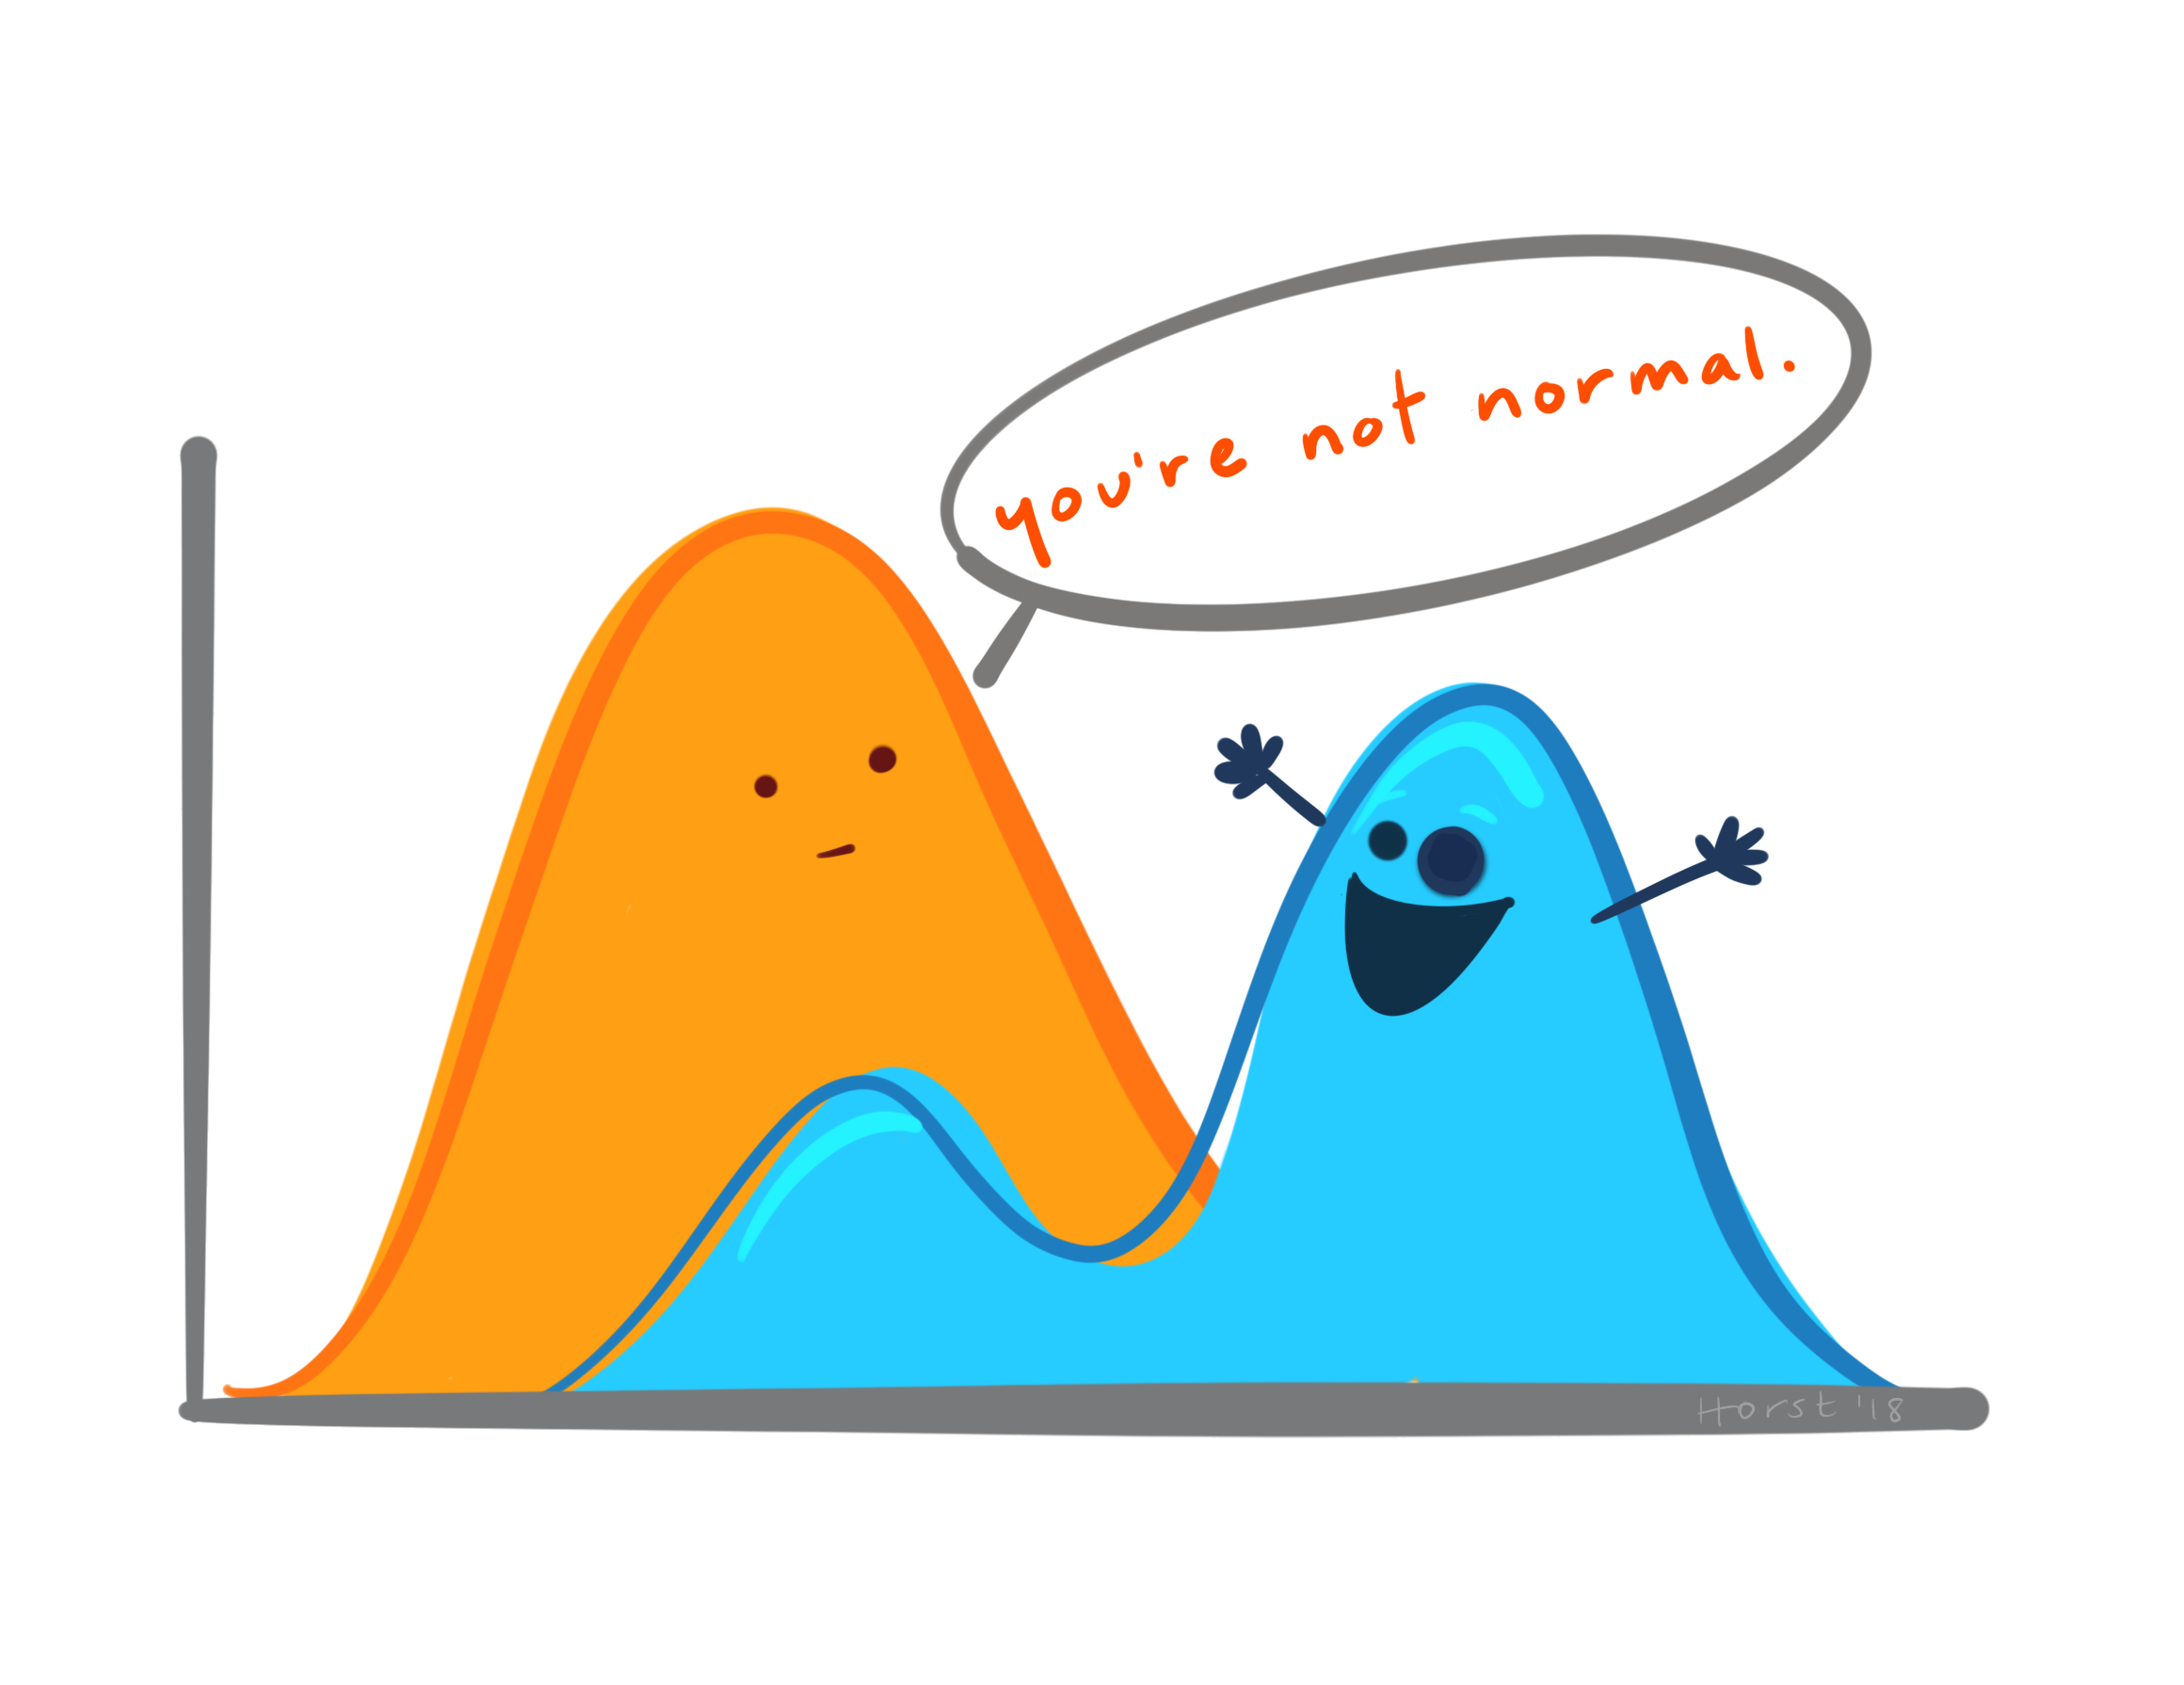
\includegraphics[width=0.9\columnwidth]{not_normal_transparent.png}
        \end{column}
    \end{columns}
\end{frame}

\subsection{Dados com \textit{Outliers}}
\begin{frame}{Dados com \textit{Outliers}}
    Modelos baseados na \textbf{distribuição normal são notoriamente "não robustos"}~
    para outliers, no sentido de que \textbf{uma única observação \textit{outlier} pode
    afetar fortemente a inferência para todos os parâmetros no modelo},
    mesmo aqueles com pouca conexão substantiva com a observação \textit{outlier}.
\end{frame}

\subsection{Superdispersão}
\begin{frame}{Superdispersão (\textit{Overdispersion})}
    \begin{defn}[Superdispersão e Subdispersão]
        A superdispersão \textit{overdispersion} e a subdispersão\footnote{bem
        mais raro no mundo real}
        \textit{underdispersion} referem-se a dados que mostram mais ou menos
        variação do que o esperado com base em um modelo de probabilidade.
        \parencite{gelman2020regression}
    \end{defn}
    \vfill
    Para cada um dos modelos padrão, há de fato uma \textbf{extensão natural} em que um
    \textbf{único} parâmetro é adicionado para permitir a superdispersão
    \parencite{gelman2013bayesian}.
\end{frame}

\begin{frame}{Exemplo de Superdispersão}
    \begin{exemplo}[Acidentes de Trânsito]
        Suponha que você esteja analisando acidentes de trânsito.
        O modelo usualmente usado nesses tipos de fenômenos é a \textbf{Regressão
        de Poisson}.
        A distribuição de Poisson possui o mesmo valor como média e variância.
        Então, se você encontrar uma variação nos dados maior que a verossimilhança Poisson
        permite, o modelo probabilístico provavelmente não conseguirá reproduzir com
        fidelidade o fenômeno modelado.
    \end{exemplo}
\end{frame}

\subsection{Versões com Superdispersão dos Modelos Probabilísticos Padrões}
\subsubsection{$t$ de Student ao invés da Normal}
\begin{frame}{$t$ de Student ao invés da Normal}
    A distribuição $t$ de Student tem uma \textbf{cauda mais longa} que a
    distribuição Normal.
    \vfill
    O que faz uma boa candidata para \textbf{acomodar observações \textit{outliers} sem
    gerar instabilidades na inferência dos parâmetros}.
    \vfill
    Do ponto de vista Bayesiano, não há nada especial na verossimilhança
    Gaussiana/Normal. É apenas uma distribuição probabilística especificada
    em um modelo. Podemos deixar o modelo mais robusto ao usarmos uma distribuição $t$
    de Student como função de verossimilhança.
\end{frame}

\begin{frame}{$t$ de Student ao invés da Normal}
    \centering
    \begin{tikzpicture}
        \begin{axis}[every axis plot, line width=2pt,
            ylabel=PDF,
            domain=-4:4,samples=200,
            axis x line*=bottom, % no box around the plot, only x and y axis
            axis y line*=left % the * suppresses the arrow tips
            ]

            \addplot [blue] {gaussian(0, 1)};
            \addlegendentry{Normal}
            \addplot [red] {student(3)};
            \addlegendentry{Student com $\nu=3$}
        \end{axis}
    \end{tikzpicture}
\end{frame}

\begin{frame}{$t$ de Student ao invés da Normal}
    Ao usarmos uma verossimilhança $t$ de Student ao invés da Normal, o erro do modelo,
    $\sigma$ não segue uma distribuição normal, mas sim uma distribuição $t$ de Student:
    $$
    \begin{aligned}
        \boldsymbol{y} &\sim \text{Student}\left( \nu, \alpha + \mathbf{X} \boldsymbol{\beta}, \sigma \right) \\
        \alpha &\sim \text{Normal}(\mu_\alpha, \sigma_\alpha) \\
        \boldsymbol{\beta} &\sim \text{Normal}(\mu_{\boldsymbol{\beta}}, \sigma_{\boldsymbol{\beta}}) \\
        \nu &\sim \text{Log-Normal}(2, 1) \\
        \sigma &\sim \text{Exponencial}(\lambda_\sigma)
    \end{aligned}
    $$
    \small
    Além disso, é apropriado incluir os graus de liberdade $\nu$ como um parâmetro a
    ser estimado pelo modelo \parencite{gelman2013bayesian}. Uma \textit{priori}
    de cauda longa e restrita a somente tomar valores positivos é adequada.
\end{frame}

\begin{frame}[fragile]{\href{https://paul-buerkner.github.io/brms/}{\texttt{brms}} -- $t$ de Student ao invés da Normal}
    \begin{lstlisting}
    brm(...
      family = @student(link = "identity")@
    )
    \end{lstlisting}
\end{frame}

\subsubsection{Beta-Binomial ao invés da Binomial}
\begin{frame}{Beta-Binomial ao invés da Binomial}
    A distribuição binomial tem uma limitação prática de que temos somente um
    parâmetro livre\footnote{já que $n$ vem dos dados} ($p$), o que implica em
    a \textbf{variância ser determinada pela média}. Isso faz com que a verossimilhança
    binomial \textbf{não} seja robusta à superdispersão.
    \vfill
    Uma alternativa robusta é a \textbf{distribuição beta-binomial}, que, como o nome
    sugere, é uma \textbf{mistura beta de binomiais}. Além disso, permite com que
    a \textbf{variância seja diferente da média}, garantindo \textbf{robustez}
    à superdispersão.
\end{frame}

\begin{frame}{Beta-Binomial ao invés da Binomial}
    A distribuição beta-binomial é uma binomial, mas a probabilidade $p$ é parametrizada
    com uma distribuição $\text{Beta}(\alpha, \beta)$. Geralmente usamos $\alpha$ como
    a probabilidade $p$ da binomial e $\beta$ é o parâmetro adicional para controlar
    superdispersão. Valores de $\beta$ iguais a $1$ fazem a beta-binomial se comportar
    igual a uma binomial.
    $$
    \begin{aligned}
        \boldsymbol{y} &\sim \text{Beta-Binomial}(n, p, \phi) \\
        p &\sim \text{Logística/Probit}(\alpha +  \mathbf{X} \boldsymbol{\beta}) \\
        \alpha &\sim \text{Normal}(\mu_\alpha, \sigma_\alpha) \\
        \boldsymbol{\beta} &\sim \text{Normal}(\mu_{\boldsymbol{\beta}}, \sigma_{\boldsymbol{\beta}}) \\
        \phi &\sim \text{Exponencial}(1)
    \end{aligned}
    $$
    \small
    É apropriado incluir o parâmetro de superdispersão $\beta$ como um parâmetro a
    ser estimado pelo modelo \parencite{gelman2013bayesian,mcelreath2020statistical}.
    Uma \textit{priori} de cauda longa e restrita a somente tomar valores positivos é
    adequada.
\end{frame}

\begin{frame}[fragile]{\href{https://paul-buerkner.github.io/brms/}{\texttt{brms}} -- Beta-Binomial ao invés da Binomial\footnote{sugiro verem \href{https://bookdown.org/content/4857/monsters-and-mixtures.html}{essa implementação Solomon Kurz}}}
    \begin{lstlisting}[basicstyle=\footnotesize]
# verossimilhanca customizada
beta_binomial2 <- @custom_family@("beta_binomial2",
  dpars = c("mu", "phi"),
  links = c("logit", "log"), lb = c(NA, 0),
  type = "int", vars = "vint1[n]")
stan_funs <- "
  real beta_binomial2_lpmf(int y, real mu, real phi, int T) {
    return beta_binomial_lpmf(y | T, mu * phi, (1 - mu) * phi);
  }
  int beta_binomial2_rng(real mu, real phi, int T) {
    return beta_binomial_rng(T, mu * phi, (1 - mu) * phi);
  }"
stanvars <- stanvar(scode = stan_funs, block = "functions")
brm(...,
  family = @beta_binomial2@,  # verossimilhanca customizada
  prior = c(..., @prior(exponential(1), class = phi@))
    \end{lstlisting}
\end{frame}

\subsubsection{$t$ de Student ao invés da Binomial}
\begin{frame}{$t$ de Student ao invés da Binomial}
    \small
    Também chamada de \textit{Robit}\footnote{há uma bela discussão com Gelman,
    Vehtari e Kurz no
    \href{https://discourse.mc-stan.org/t/robit-regression-not-robust/21245/}{
        \textit{discourse} do \texttt{Stan}}} \parencite{gelman2013bayesian, gelman2020regression}.
    A ideia é "robustizar"~ a regressão logística com uma formulação usando dados
    latentes $z$ e dar uma uma distribução $t$ de Student aos erros latentes $\epsilon$:
    $$
    \begin{aligned}
        y_i & = \begin{cases} 0 & \text{se } z_i < 0 \\ 1 & \text{se }\ z_i > 0 \end{cases}\\
        z_i & = X_i \boldsymbol{\beta} + \epsilon_i \\
        \epsilon_i &\sim \text{Student} \left (\nu, 0, \sqrt{\frac{\nu - 2}{\nu}} \right) \\
        \nu &\sim \text{Gamma}(2, 0.1) \in \left[2, \infty \right)
    \end{aligned}
    $$
    \footnotesize
    O grande segredo aqui é usar uma distribuição Gamma como \textit{priori}
    dos graus de liberdade $\nu$ truncada para valor mínimo de $\nu = 2$. Outra opção
    é literalmente especificar $\nu=4$.
\end{frame}

\begin{frame}[fragile]{\href{https://paul-buerkner.github.io/brms/}{\texttt{brms}} -- $t$ de Student ao invés da Binomial}
    \begin{lstlisting}[basicstyle=\footnotesize]
stan_inv_robit <- "
real inv_robit(real y, real nu) {
    return(student_t_cdf(y, nu, 0, sqrt((nu - 2) / nu)));
    }"
stanvar_inv_robit <- stanvar(scode = stan_inv_robit, block = "functions")
robit_formula <-
bf(y_c | trials(1) ~ inv_robit(eta, nu),
    nlf(eta ~ b0 + b1 * x),
    b0 + b1 ~ 1,
    nu ~ 1,
    nl = TRUE)
brm(formula = robit_formula,
    family = @binomial("identity")@,
    formula = robit_formula,
    prior = c(prior(normal(0, 1), nlpar = b0),
    prior(normal(0, 1), nlpar = b1),
    prior(gamma(2, 0.1), nlpar = nu, @lb = 2@)),
    stanvars = stanvar_inv_robit)
    \end{lstlisting}
\end{frame}

\subsubsection{Binomial Negativa ao invés de Poisson}
\begin{frame}{Binomial Negativa ao invés de Poisson}
    Esse é o exemplo que falamos sobre superdispersão.
    A distribuição de Poisson possui o mesmo valor como média e variância.
    \vfill
    Então, se você encontrar superdispersão, provavelmente precisará de uma alternativa
    robusta à Poisson. Aqui que entra a binomial negativa que "robustiza"~
    a Poisson com um parâmetro extra $\phi$.
    \vfill
    Esse parâmetro é a probabilidade de sucessos $p$ da distribuição binomial negativa
    e geralmente usamos uma distribuição gamma como \textit{priori} para que $\phi$
    cumpra a função de um parâmetro de~"dispersão recíproca".
\end{frame}

\begin{frame}{Binomial Negativa ao invés de Poisson}
    $$
    \begin{aligned}
    \boldsymbol{y} &\sim \text{Binomial Negativa} \left( e^{(\alpha + \mathbf{X} \boldsymbol{\beta})}, \phi \right) \\
    \phi &\sim \text{Gamma}(0.01, 0.01) \\
    \alpha &\sim \text{Normal}(\mu_\alpha, \sigma_\alpha) \\
    \boldsymbol{\beta} &\sim \text{Normal}(\mu_{\boldsymbol{\beta}}, \sigma_{\boldsymbol{\beta}})
    \end{aligned}
    $$
    A ideia é dar uma \textit{priori} cauda longa para $\phi$, algo como
    $\text{Gamma}(0.01, 0.01)$ funciona.
\end{frame}

\begin{frame}[fragile]{\href{https://paul-buerkner.github.io/brms/}{\texttt{brms}} -- Binomial Negativa ao invés de Poisson}
    \begin{lstlisting}
    brm(...
      family = @negbinomial(link = "log")@
    )
    \end{lstlisting}
\end{frame}

\subsubsection{Mistura de Binomial Negativa ao invés de Poisson}
\begin{frame}{Mistura de Binomial Negativa ao invés de Poisson}
    \small
    Mesmo usando uma binomial negativa, caso a superdispersão seja muito acentuada,
    em especial quando temos muita \textbf{inflação de zeros} (\textit{zero-inflated}),
    o seu modelo ainda pode resultar em patologias.
    Uma outra sugestão é usar uma mistura de binomial negativa \parencite{mcelreath2020statistical}.
    Aqui, $S_i$ é uma variável binária (\textit{dummy})
    indicando se a observação $i$ tem valor diferente de zero ou não.
    $S_i$ pode ser modelado usando uma regressão logística:
    $$
    \begin{aligned}
    \boldsymbol{y}
    & \begin{cases}
        = 0, &\text{ se } S_i = 0 \\
        \sim \text{Binomial Negativa} \left( e^{(\alpha + \mathbf{X} \boldsymbol{\beta})}, \phi \right), &\text{ se } S_i = 1
    \end{cases} \\
    P(S_i = 1) &= \text{Logística/Logit}(\mathbf{X} \boldsymbol{\gamma}) \\
    \boldsymbol{\gamma} &\sim \text{Beta}(1, 1)
    \end{aligned}
    $$
    \small
    $\boldsymbol{\gamma}$ é um novo conjunto de coeficientes para essa parte do modelo com
    \textit{prioris} uniformes de $\text{Beta} (1, 1)$.
\end{frame}

\begin{frame}[fragile]{\href{https://paul-buerkner.github.io/brms/}{\texttt{brms}} -- Mistura de Binomial Negativa ao invés de Poisson}
    \begin{lstlisting}
    brm(...
      family = @zero_inflated_negbinomial(link = "log")@,
      prior = c(
          ...
        @prior(gamma(0.01, 0.01), class = shape)@,
        @prior(beta(1, 1), class = zi)@
    ))
    \end{lstlisting}
\end{frame}

\subsection{Por quê usar Modelos Não-Robustos?}
\begin{frame}{Por quê usar Modelos Não-Robustos?}
    O \textbf{teorema do limite central} nos diz que a distribuição \textbf{normal}
    é uma modelo apropriado para dados que são formados como a \textbf{soma de um grande número
    de componentes independentes}.
    \vfill
    Mesmo quando não estão naturalmente implícitos na estrutura de um problema,
    os \textbf{modelos simples não-robustos são computacionalmente convenientes}.
    \vfill
    Claro o que deve sempre guiar a sua escolha de modelo, além da natureza específica
    do processo de geração de dados do fenômeno que você está estudando, é
    a \textbf{verificação preditiva da posterior}.
\end{frame}
